\chapter{Technology Computer Aided Design Simulations}
\label{chap:TCAD}
In this Chapter the basics of Technology Computer Aided Design, {\it TCAD}, simulations will be given. 
After introducing TCAD simulation tools (Section~\ref{sec:TCADIntro}) and explaining their importance
 for the development of silicon detectors for HEP applications, some examples of TCAD based 
 studies will be given, both for sensor design optimisation and sensor simulation 
 (Sections~\ref{sec:sensordesign} and~\ref{sec:sensorsimulation}). 
Section~\ref{sec:TCADRadDamage} will be devoted to the modellisation of radiation damage in 
TCAD simulation, a topic of very large interest in view of the new trackers for the 
the High Luminosity phase of the Large Hadron Collider (more details in Chapter~\ref{chap:ITk}).

\section{Introduction}
\label{sec:TCADIntro}

 TCAD is a branch of electronic design automation that models semiconductor fabrication and 
 semiconductor device operation. 
 The modelling of the fabrication is termed Process TCAD, while the modelling of the device operation 
 is termed Device TCAD. 
Included are the modelling of process steps (such as diffusion and ion implantation), and modelling of 
the behaviour of the electrical devices based on fundamental physics, such as the doping profiles of 
the devices. 

The advantages TCAD based studies offer during the development of semiconductor sensors 
and electronics are multiple: 

\begin{itemize}
\item they are predictive
\item they provide insight
\item they capture and visualise theoretical knowledge
\end{itemize}

TCAD based studies are predictive since they offer the possibility to explore alterative~/~innovative 
solutions providing quantitative predictions, allowing to test new hypothesis. 
They also offer insight: they allow the user to explore physical quantities otherwise impossible to 
access in reality, like point-by-point carriers distribution, electric field lines, etc. In this sense they 
are also a powerful tool to learn semiconductor physics, provided a good base knowledge is present.
Finally TCAD tools make it possible to literally visualise new ideas and the results they promise to 
offer.

In the following some examples of TCAD based sensor design and of predictions for HEP
trackers will be given.

\section{Sensor Design}
\label{sec:sensordesign}

The possibility to explore several designs for a silicon detector without having to realise them is 
of course an asset since it allows to reduce the number of submissions, allowing to save time 
and money. 
One example of such studies is given by the optimisation of the detector edge design. 
As already discussed in Section~\ref{sec:pads} it is important to control the voltage 
drop from one side of the junction to the other one. This is particularly true for nowadays 
silicon sensors where, to maximise the detector acceptance, the dead area at the 
detector edge has to be kept at minimum (see also~\ref{sec:edgeless}). One way to achieve 
small dead areas and and at the same time avoid large electric fields is to add several 
guard rings (GRs) that surround the sensitive area of the sensor. How many GRs include in 
the detector, how large their implants should be, which total area they should cover are 
some of the questions that TCAD simulations can address. 

In order for the answers to be really reliable it is important to have access to information 
like the doping profiles of the various detector implants. This is often not possible, since 
the silicon foundries don't disclose these information. Some {\it a posteriori} analysis is possible, 
like Secondary Ion Mass Spectroscopy, {\it SIMS}. SIMS is a vacuum based technique 
which relies on the bombardment of a sample surface with a primary ion 
beam  followed  by  mass  spectrometry  of  the 
 emitted  ionised  secondary  ions.  For SIMS see for example~\cite{dinu:tel-00872318}.
A result of the SIMS investigation~\cite{SIMS} of a {\it p-spray} doping is shown in Figure~\ref{fig:sims_pspray}. 

\begin{figure}[!htbp]
\centering
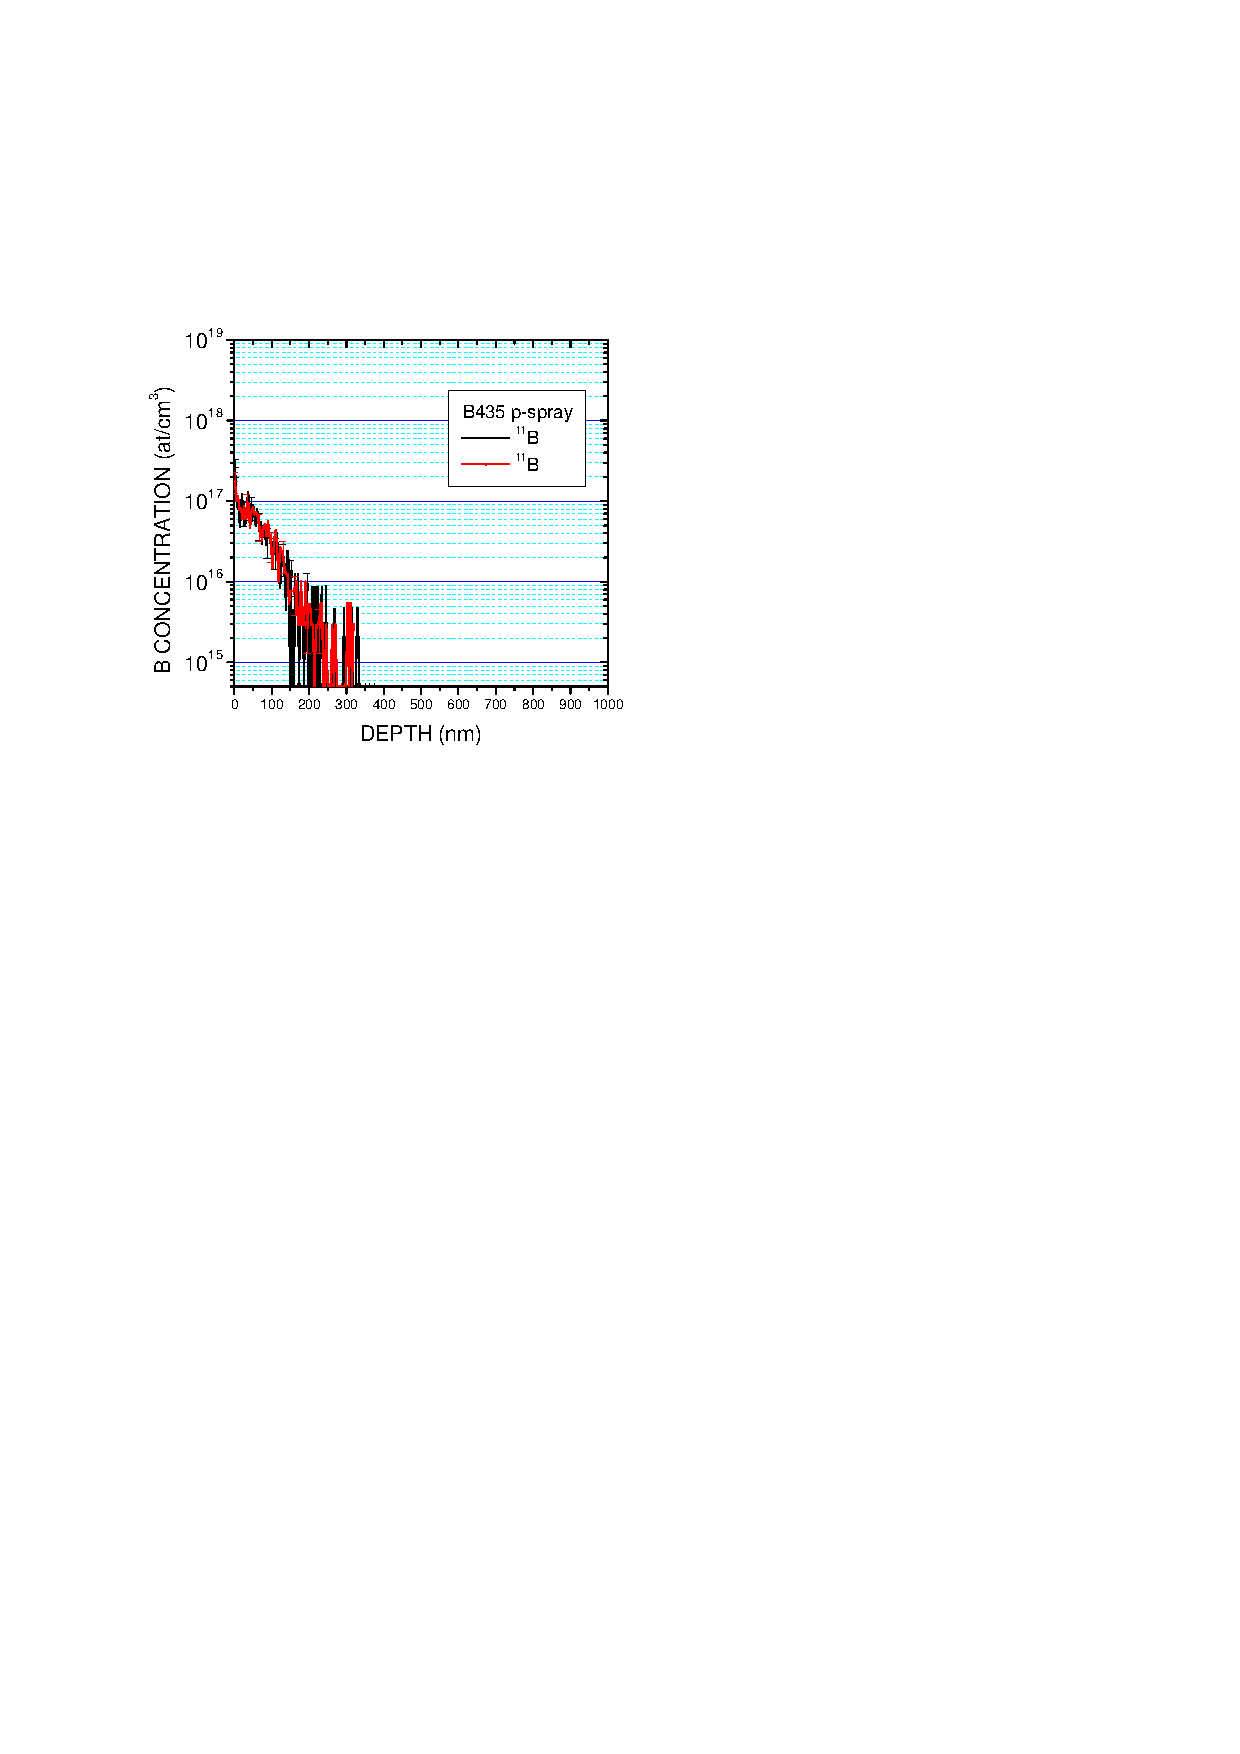
\includegraphics[width=0.65\textwidth]{sims_pspray.pdf}
\caption{\label{fig:sims_pspray}Boron depth profiles obtained in two points for each {\it p-spray} area 
on samples taken from an $n-on-p$ production.}
\end{figure}

P-spray is needed to counter the accumulation of electrons between $n^+$ implants in an 
electron collecting detector, which otherwise would short the electrodes and degrade the 
detector performance. The positive oxide charge is the responsible for the electron layer 
at the Si-SiO$_2$ interface~\cite{Lutz:411172}. 

Thanks to inputs like the ones from SIMS it is possible to make optimal choices for the detector 
edge design as it was done for the edgeless pixels sensors reported in~\cite{bib:nim2012}. 
An example of the agreement between real data and TCAD simulations is shown in 
Figure~\ref{fig:IV_BD}.
\begin{figure}[!htbp]
\centering
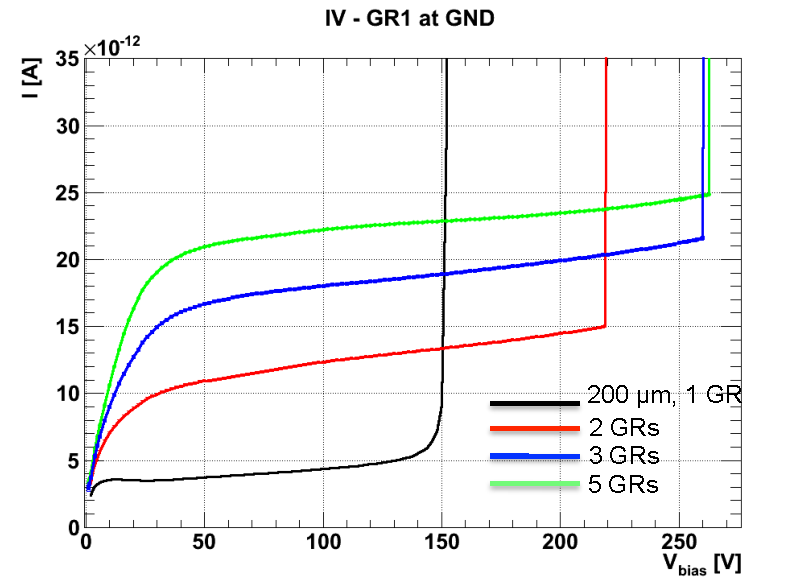
\includegraphics[width=0.5\textwidth]{IV_simulations}
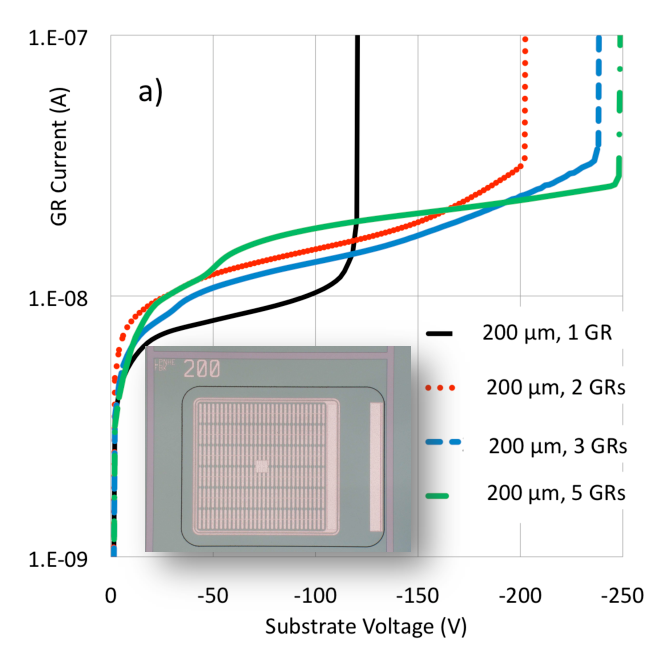
\includegraphics[width=0.39\textwidth]{IV_data}
\caption{\label{fig:IV_BD}IV curves for edgeless $n-on-p$ pixel test structures. (left) TCAD simulations 
(right) Real data from~\cite{bib:nim2012}. Detectors with the same pixel-to-edge minimal distance 
and different number of GRs are compared. In the right figure a photo of the tested detector is 
shown in the inset.}
\end{figure}
In the Figure the IV curves of edgeless $n-on-p$ pixel test structures are compared. The 
parameter of interest here is the breakdown (BD) voltage, which in the presence of 
p-spray depends critically on the dose of the implant and on the shape of the electrode 
on top of the $n^+$ implant. 

As it can be seen for what concerns the BD voltage the level of agreement between real data 
and TCAD simulations is at 20\% or better. This was an important achievement since 
the designs of the real sensors was driven by the TCAD simulations studies; they allowed 
to choose among different possible combinations of minimal pixel-to-edge distances and 
number of GRs. 

A similar studied, reported in Figure~\ref{fig:width_GRs}, showed that keeping the number of GRs fixed and simply increasing the 
minimal pixel-to-edge distance doesn't make the BD voltage larger.

\begin{figure}[!htbp]
\centering
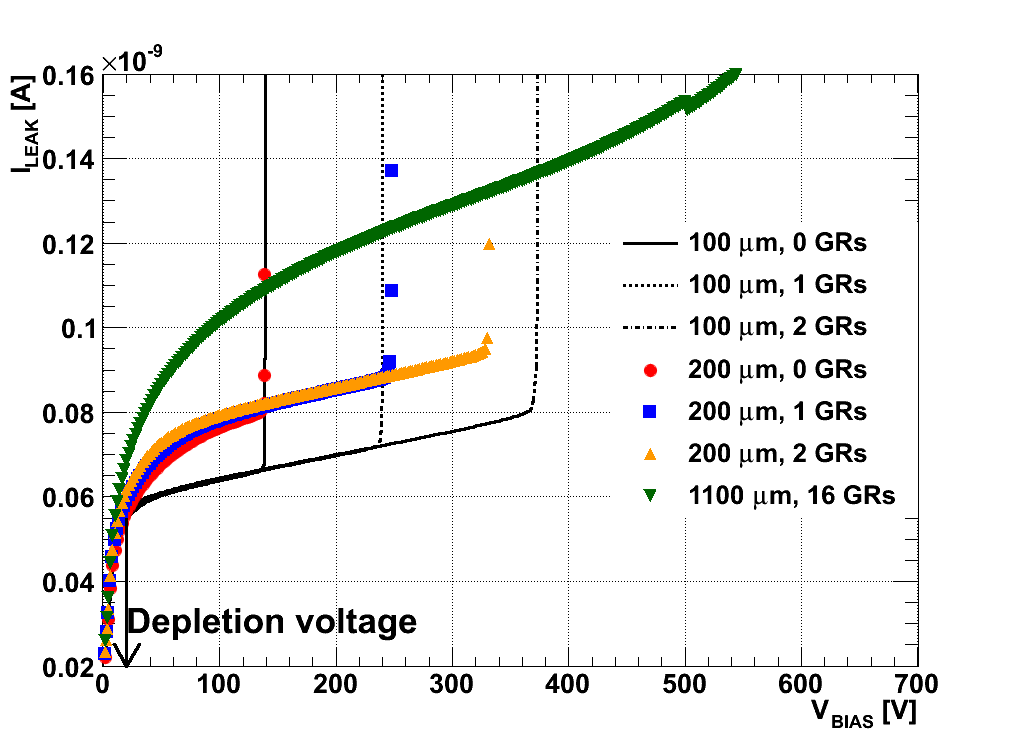
\includegraphics[width=0.65\textwidth]{edgeless_BD_FL0_BandW_mix}
\caption{\label{fig:width_GRs}Simulated IV curves for edgeless $n-on-p$ pixel test structures. Detectors with different pixel-to-edge minimal distance 
and different number of GRs are compared.}
\end{figure}

This effect is due to the p-spray which is equipotential till it doesn't cross a $n^+$ implant, like a 
GR or the pixels. Hence, increasing the distance between the detector edge and the pixels but 
not adding more GRs doesn't allow a more smooth voltage drop, hence doesn't change the 
BD voltage. The fact the p-spray is equipotential was verified during the simulation studies, a test 
otherwise difficult to accomplish.


The one presented so far is a very simple but effective case in which TCAD simulations drive the 
sensors design. More sophisticated studies can be carried out, in which processes like 
etching, oxide growing, doping implantation and diffusion and many more can be simulated. 
These kind of studies are beyond the scope of this report; an example of such studies 
can be found in~\cite{CISSIMDET2014}. 

\section{Sensor Simulation}
\label{sec:sensorsimulation}

Sensor simulation allows to study the detector behaviour under numerous conditions like 
forward~/~reverse voltage, application of sinusoidal signals on electrodes, illumination with lasers or 
generally light, generation of charge in the 
bulk by charged particles, radiation induced traps in the bulk and at the surface, low temperature 
operation, etc., 
and of course combination of them.
All these correspond to working condition for HEP detectors, hence predictions can be extracted 
for example for a heavily irradiated silicon detector in terms of charge collection efficiency, operating 
voltage and leakage current level.

Again such studies allow to make detector choices that save money and time and give access to 
quantities like carriers distribution otherwise impossible to measure. An example is given in 
Figure~\ref{fig:carr_conc}, where the result of 2D simulations of an  $n-on-p$ detector 
are reported.

\begin{figure}[!htbp]
\centering
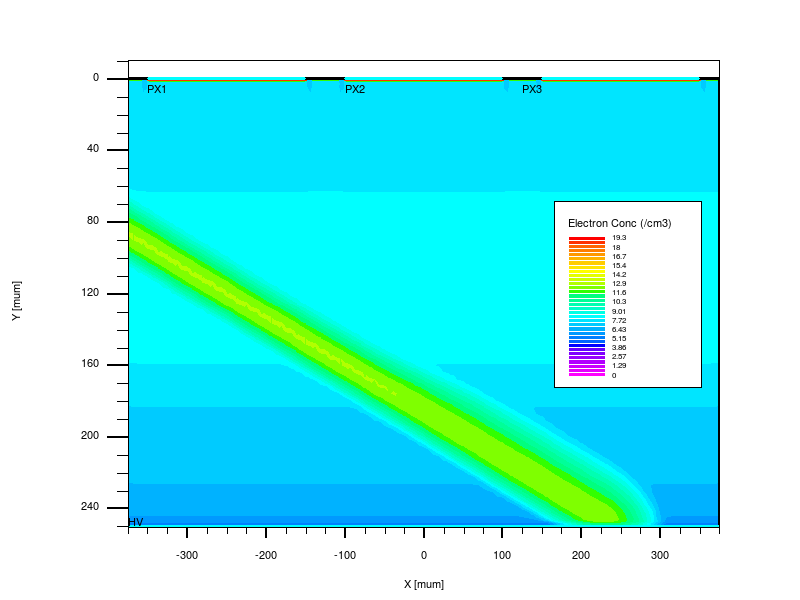
\includegraphics[width=0.45\textwidth]{econ_early.png}
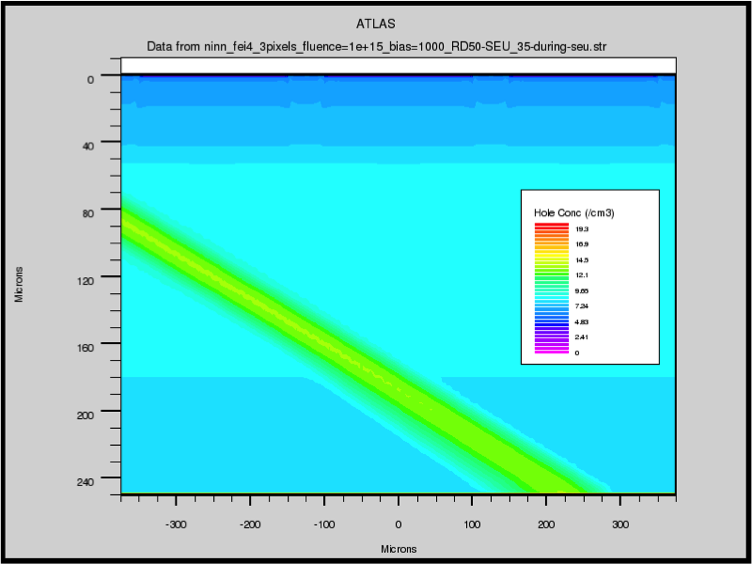
\includegraphics[width=0.45\textwidth]{hcon_early.png}
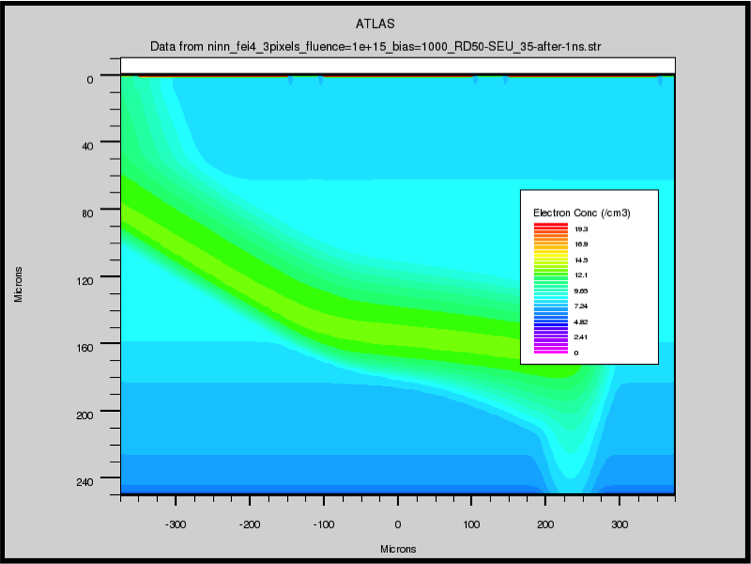
\includegraphics[width=0.45\textwidth]{econ_late.png}
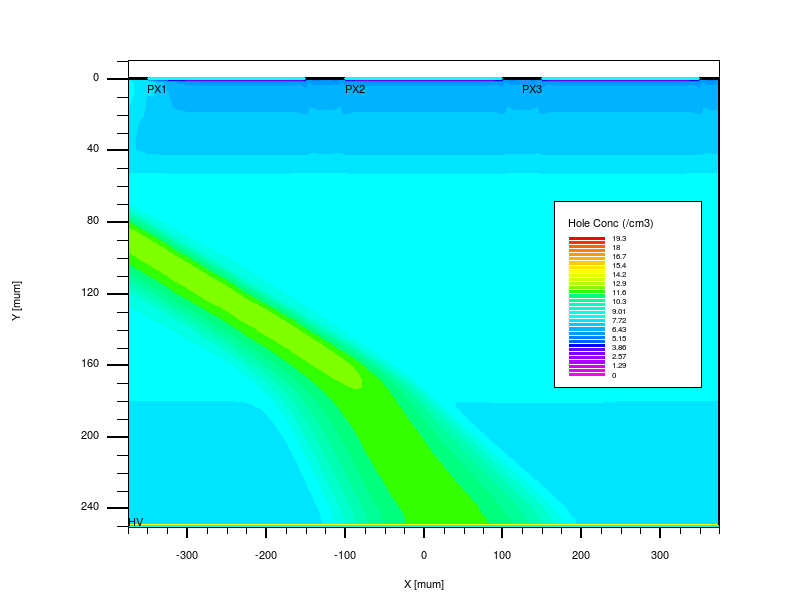
\includegraphics[width=0.45\textwidth]{hcon_late.png}
\caption{\label{fig:carr_conc}2D simulations of an $n-on-p$ detector. Carriers concentration
are reported when the detector is over depleted and a MIP stroke at $t=0$~s. 
(Top) Carriers distribution during the MIP strike. (Bottom) After 1~ns. (Left) electron concentration. 
(Right) Hole concentration. MIP was impinging at 20$^{\circ}$ with respect to the sensor surface.}
\end{figure}

Three collecting electrodes are simulated; the detector is 250~$\mu$m thick and the pitch 
is 250~$\mu$m. The detector is hit my a MIP when it is in over-depletion; the MIP strikes at 
an angle of 20$^{\circ}$ with respect to the sensor surface. The detector was simulated after 
an irradiation fluence of $\Phi=1\times10^{15}$~n$_{\rm eq}$/cm$^2$
It can be seen from the Figure that electrons drift faster than holes; a large fraction of holes 
have moved little from the original position while electrons have gained much more distance 
after 1~ns. 

This kind of simulation are needed to interpret data from test beams when tracks are impinging 
at shallow angle. The charge profile in data can be compared over the signal amplitude from pixels in 
long clusters to the one predicted by TCAD simulations; this will allow to infer the electric field 
distribution inside the irradiated detector thanks to so-called {\it grazing angle} 
technique~\cite{Henrich:687041,Lari:2001qqa}; more 
on this in the next Section.

In case of edgeless sensors it is interesting to investigate the charge collection efficiency (CCE) 
in the un-instrumented area between the last collecting electrode and the detector edge. 
Other than the BD voltage, also CCE is an important factor on which optimise the 
detector design. In Figure~\ref{fig:Edgeless_CCE} the result of a simulation study for an 
$n-on-p$ edgeless detector 
\begin{figure}[!htbp]
\centering
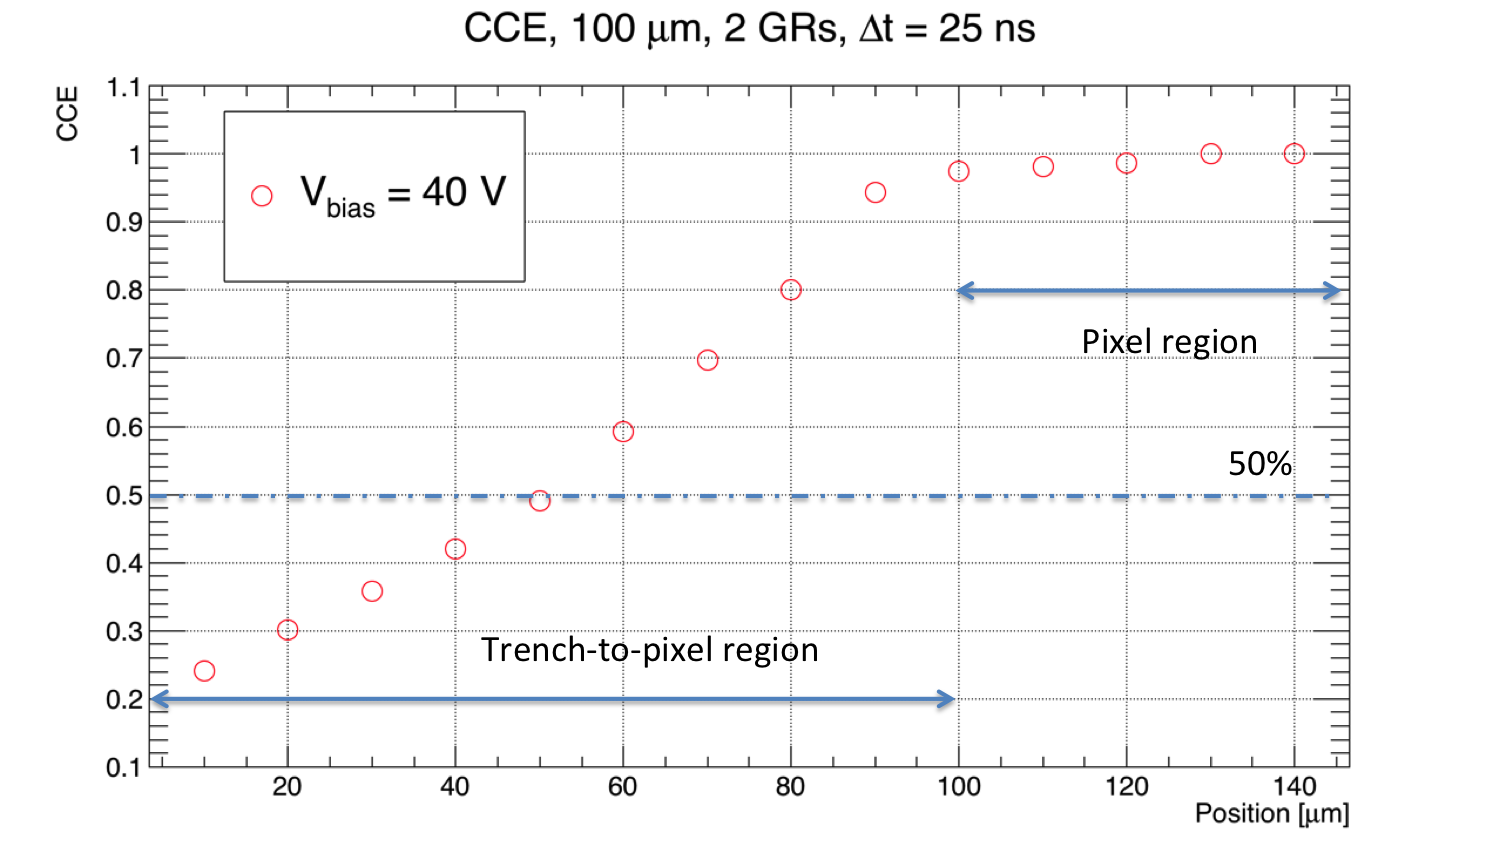
\includegraphics[width=0.65\textwidth]{Edgeless_CCE.png}
\caption{\label{fig:Edgeless_CCE}Simulated CCE as a function of the MIP impact point. 
It is the result of a 2D simulations of an $n-on-p$ edgeless detector. The bias voltage and the integration time 
are indicated.}
\end{figure}

The simulations indicate that it is possible to collect at least 50\% of the signal amplitude for a MIP 
up to 50~$\mu$m away from the last collecting electrode. This is very promising for {\it active edge} 
detectors  (see also~\ref{sec:edgeless}).

\section{Discussion on Fundamental Parameters and TCAD Simulations}
The two most used commercial TCAD products in the HEP community are Silvaco\footnote{\url{https://www.silvaco.com/products/tcad.html}} and Synopsys\footnote{\url{https://www.synopsys.com/silicon/tcad.html}}.

In a test to see how much the two products differ in terms of physics models it turned out 
that at least in two fundamental semiconductor physics observables they were quite far apart. 
The result of the investigations are documented in~\cite{bomben_rd50_Torino}.

The first observable under investigation was the thermal velocities of the carriers. The results 
are illustrated in Figure~\ref{fig:vtherm}.

\begin{figure}[!htbp]
\centering
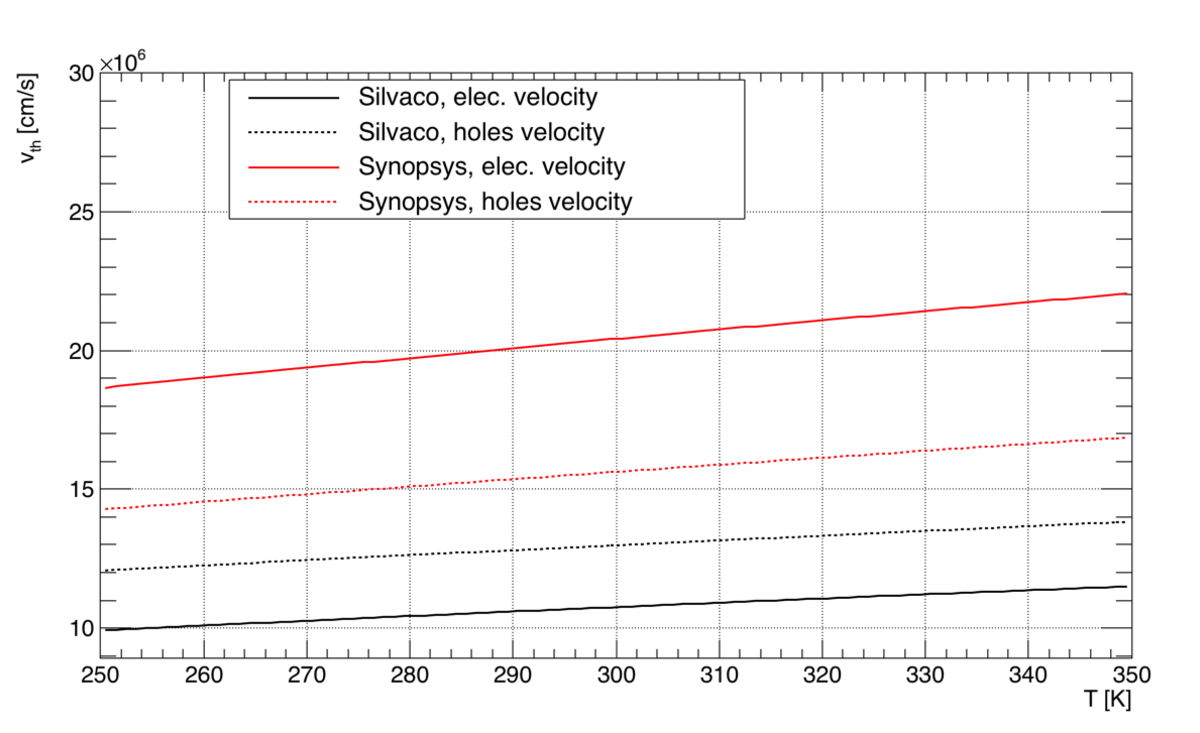
\includegraphics[width=0.65\textwidth]{vtherm}
\caption{\label{fig:vtherm}Carrier thermal velocities as a function of the temperature.}
\end{figure}
As it can be seen there is almost a factor of 2 of difference between the two tools for the electrons 
thermal velocities. The reason for this disagreement has to be found in the carriers  mass value
used in the thermal velocities calculation. While Synopsys uses the effective  mass derived 
from the energy band curvature, Silvaco inserts the rest mass of the electron. 
Such a difference in the  carriers thermal velocities affect the carriers transport phenomena, 
the leakage current level and the effects due to radiation damage defects. 
 
 The second parameter that was investigated was the bandgap energy $E_g$. The default value in 
 Silvaco for $E_g$ at $T=$300~K is of 1.08~eV. This is surprisingly low compared to values in literature 
 (see for example~\cite{Lutz:411172,Sze1981,Wang1989,Shockley}) which are comprised 
 in the range 1.11-1.12~eV.
The temperature dependence of $E_g$ is based on~\cite{Sze1981}:
\begin{equation}
E_g(T)=E_g(0) -\dfrac{\alpha T^2}{T+\beta}=E_g(300)+\alpha\Bigg[ \dfrac{(300)^2}{300+\beta}-\dfrac{T^2}{T+\beta}  \Bigg] \equiv E_g(T_{ref})+\alpha\Bigg[ \dfrac{(T_{ref})^2}{T_{ref}+\beta}-\dfrac{T^2}{T+\beta}  \Bigg] 
\label{eq:EgT}
\end{equation}
where $T_{ref}$ is some reference temperature.
Both TCAD products agree on the $\alpha$ and $\beta$ parameters values:

\begin{table}[!htbp]
\caption{\label{eq:Egalphabeta}Parameter values for the temperature dependence of the bandgap. 
See also Equation~\ref{eq:EgT}}
\centering
\begin{tabular}{|c|c|}
\hline
parameter & value \\
\hline 
$\alpha$ & 4.73$\times$10$^{-4}$~eV/K \\
\hline 
$\beta$ & 636~K \\
\hline
\end{tabular}
\end{table}

Silvaco tools are built on the value $E^{Sil}_g(300)=$1.08~eV while Synopsys on $E^{Syn}_g(0)=$1.1696~eV. 
Extrapolating $E_g^{Syn}(0)$ to $T=$300K from the one gets the expected 
$E_g^{Syn}(300)\sim$1.12~eV, in agreement with literature.

Silvaco developers explained\footnote{private communication} the abnormal $E^{Sil}_g(300)$ value 
because of very low resistivity 
Silicon wafers used to estimate the bandgap energy when their TCAD tool was developed. 
They are aware of the issue and claim that the Silvaco TCAD tools are anyhow consistent with 
the $E^{Sil}_g(300)$ value chosen and predictions are reliable. The 

To test the latter statement the $E^{Sil}_g(300)$ value was changed in the simulation package, 
and results compared. 
A 200~$\mu$m thick, 50~$\mu$m wide $n-on-p$ diode was simulated using Silvaco 2D device 
simulator. Temperature was varied between -20$^{\circ}$ and +20$^{\circ}$ in 5$^{\circ}$ steps. 
Several scenarios have been invetigated:

\begin{itemize}
\item[\bf default] using default Silvaco parameters values
\item[\bf EG112] setting $E^{Sil}_g(300)=1.12$~eV
\item[\bf Syn. Th. Vel.] setting thermal velocities to the values used by Synopsys tool
\item[\bf EG112 \& Syn. Th. Vel.] combination of the two above 
\item[\bf NO BGN] turning off the model for bandgap narrowing based on the concentrations~\cite{SLOTBOOM1977279}.
\end{itemize}

Several studies were performed which will now be discussed.

\subsubsection{Leakage Current Level}




In Figure~\ref{fig:ILeak20C} a comparison of the simulated leakage current in the five scenarios for $t=20^{\circ}$C is presented.
\begin{figure}[!htbp]
\centering
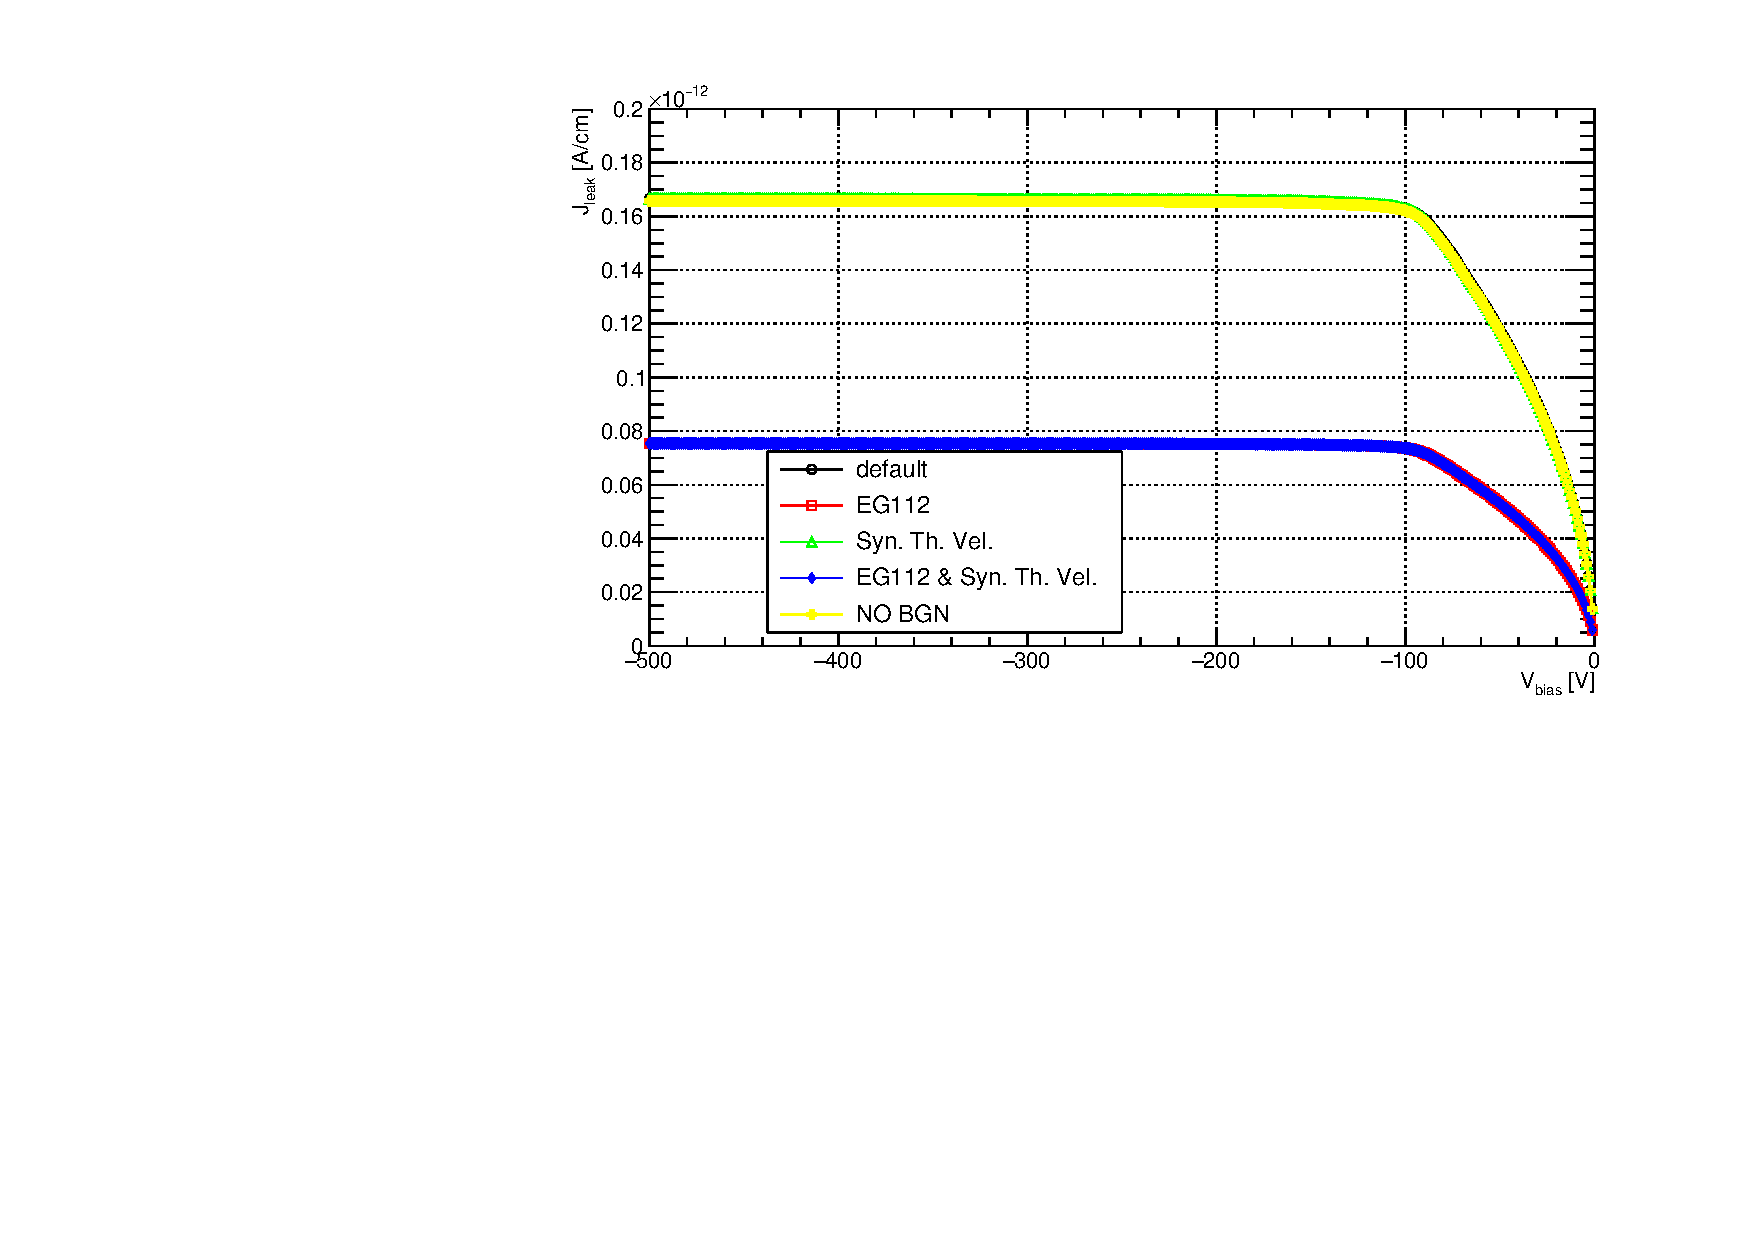
\includegraphics[width=0.65\textwidth]{currents_T20_scenarios.pdf}
\caption{\label{fig:ILeak20C}Simulated current density as a function of the bias voltage for different 
scenarios at $t=20^{\circ}$C. See text for more details.}
\end{figure}
It is evident that the only parameter playing a major role, as expected, is the bandgap energy $E^{Sil}_g(300)$. 



To verify the validity of leakage current level  from Silvaco tools the result at $V_{op}$ bias 
were compared with the theoretical value evaluated using~\ref{eq:Ileak2}. Assuming the same value
for generation and recombination lifetimes and taking the intrinsic concentration value $n_i$ from 
the simulation itself a current density of $J\sim1.6\times10^{-13}$~A/cm is expected, which 
is in excellent agreement with the value observed in simulations when the default value of 
$E^{Sil}_g(300)$ is chose ({\it i.e.} 1.08~eV); on the contrary, as it can be seen from Figure~\ref{fig:ILeak20C}, when $E^{Sil}_g(300)$ is set to 1.12~eV the simulation results don't match 
the theoretical expected values.

It has to be noted that  the simulated current is purely bulk generated; this is also clear from 
Figure~\ref{fig:ILeak20C}: the current level is stable after the depletion voltage. This feature 
is not realistic~\cite{CALZOLARI19721003} but for the sake of understing bulk generated 
current properties in TCAD simulations is very well suited since it allows to study the 
phenomenon without having to deconvolve from the current surface effects, trap assisted tunnelling 
and others.

\subsubsection{Temperature Dependence of Simulated Leakage Current}

For all temperature $T$ times scenario $S$ combination the leakage current $I_{leak}(V_{op};T;S)$ at a 
operational voltage 
$V_{op}$ defined as:

\begin{equation}
V_{op}=V_{depl}+50\,{\rm V}
\label{eq:Vop}
\end{equation} 
was extracted. It was verified that the depletion voltage $V_{depl}$ didn't depend on scenarios nor temperatures.

 The leakage current was then studied as a function of the reciprocal of the 
temperature and fitted with a function inspired by Equation~\ref{eq:IleakT}:

\begin{equation}
I = I_{ref}\Bigg(\dfrac{T}{T_{ref}}\Bigg)^n exp^{\Bigg[ -\dfrac{E_{a}}{2k_B}\Bigg( \dfrac{1}{T}- \dfrac{1}{T_{ref}} \Bigg) \Bigg]}
\label{eq:ITfunc}
\end{equation}
where $n$ and $E_{a}$ are free parameters, $I_{ref}$ the simulated current at the reference 
temperature $T_{ref}$ and $k_B$ the Boltzmann constant.

\section{Modelling Radiation Damage in TCAD Simulations}
\label{sec:TCADRadDamage}

\section{Summary}
\label{sec:TCADSummary}
